
\section{What is OSI?}
\begin{figure}[h]
    \centering
    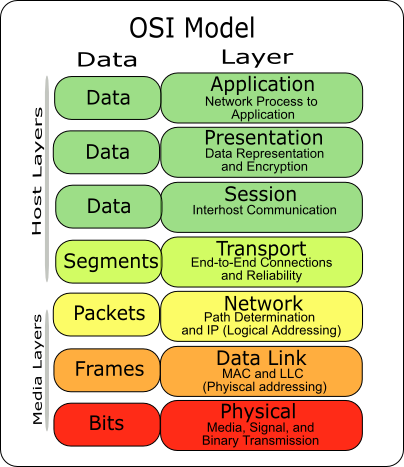
\includegraphics[width=.3\textwidth]{assets/osi/layers.png}
    \caption{The OSI Model Layers}\label{fig:osi_layers_intro}
\end{figure}
From chaos to order, the Open Systems Interconnection (OSI) model is a framework we use to understand how different networking protocols interact. 

It breaks down the complex process of network communication into seven manageable layers, each with its own specific function.

\begin{table}[h]
    \centering
    \begin{tabular}{|c|c|c|}
        \hline
        \textbf{Layer} & \textbf{Function} & \textbf{Protocols} \\
        \hline
        Application & User interface & HTTP, FTP \\
        Presentation & Data translation & SSL/TLS \\
        Session & Session management & NetBIOS \\
        Transport & Data transfer & TCP, UDP \\
        Network & Routing & IP, ICMP \\
        Data Link & Node-to-node transfer & Ethernet \\
        Physical & Bit transmission & USB \\
        \hline
        \end{tabular}
    \caption{The Seven Layers of the OSI Model}\label{tab:osi_layers}
\end{table}

We will cover these layers by example in the next chapters, drilling down into layer-specific protocols and their intersections.
